%!TEX root = ../../thesis.tex

\subsection{Data quality}
\label{sec:selection:quality}

The \pp dataset (see \Section~\ref{sec:dataset:dataset}) is hierarchically split into 
\textit{periods} of broadly consistent beam conditions, \textit{runs} typically 
corresponding to LHC fills, and \textit{luminosity blocks} of \about 2~minutes where the 
instantaneous luminosity is approximately constant. Luminosity blocks are included in the 
analysis if the detector was operating sufficiently for the recorded data to be 
considered `good for physics' (see \Figure~\ref{fig:dataset:lumi}).\footnote{
	ATLAS good runs list: \texttt{data12\symbol{95}8TeV.periodAllYear\symbol{95}DetStatus-v61-pro14-02\symbol{95}DQDefects-00-01
	-00\symbol{95}PHYS\symbol{95}StandardGRL\symbol{95}All\symbol{95}Good.xml}
} 
This corresponds to a total integrated luminosity of \unit{20.3}{\invfb}.

Individual events are vetoed if certain data quality criteria are failed:
\begin{itemize}[noitemsep,nolistsep]
	\item a noise burst in the LAr calorimeter,
	\item data corruption caused by a restart of the synchronisation system,
	\item a \textit{looser} jet is reconstructed with \pt $>$ \unit{20}{\GeV} (indicative of an HCal spike),
	\item a jet is reconstructed near a `hot' HCal tile (1st -- 8th May 2012 only).
\end{itemize}
A further quality criterion requires that the primary vertex considered as the hard 
scatter (that with the highest $\sum p_{\text{T}}^2$) must be associated with at least 
three tracks.



\subsection{Trigger}
\label{sec:selection:trigger}

It is infeasible to record all events in the \unit{20.3}{\invfb} dataset; ATLAS instead 
employs a trigger system to identify and record interesting events (see 
\Section~\ref{sec:atlas:trig}). In the \HWWlvlv search it is natural to trigger on 
high-\pt leptons, using algorithms similar to, though less sophisticated than, those in 
\Section~\ref{sec:objects:electrons} and \Section~\ref{sec:objects:muons}.

A trigger is characterised by its efficiency versus \pt curve (though it also depends on 
$\eta$), which has a turn-on followed by a plateau, as shown in 
\Figure~\ref{fig:sel:trig_eff}. It is preferable to operate on the plateau, where the 
efficiency is more stable. To maximise the signal yield, it is desirable to use a trigger 
with a lower turn-on \pt. However, increased backgrounds and limitations to trigger 
latency and bandwidth require a compromise to be found. The lowest unprescaled\footnote{
	A \textit{prescaled} trigger reduces the turn-on \pt by recording only 1 in $N$ 
	events passing the trigger, and weighting such events by a factor $N$. In doing so, 
	some statistical power is lost.
}
single lepton triggers available in 2012 had nominal \pt thresholds of \unit{24}{\GeV}. 
Fortunately, it is possible to recover trigger efficiency at low-\pt by using dilepton 
triggers, because the backgrounds are much smaller.

\begin{figure}
	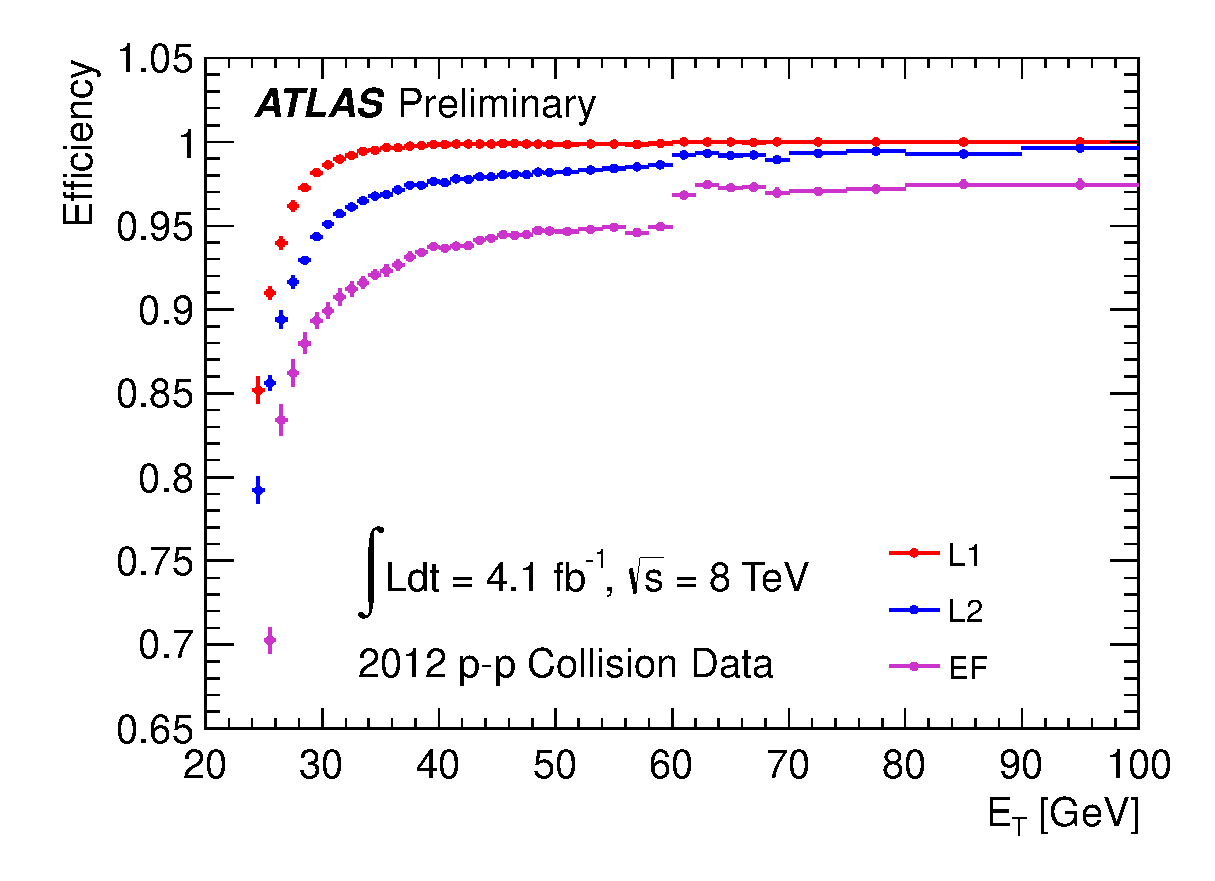
\includegraphics[width=0.495\textwidth]{tex/selection/trigger_eff_el}
	\hfill
	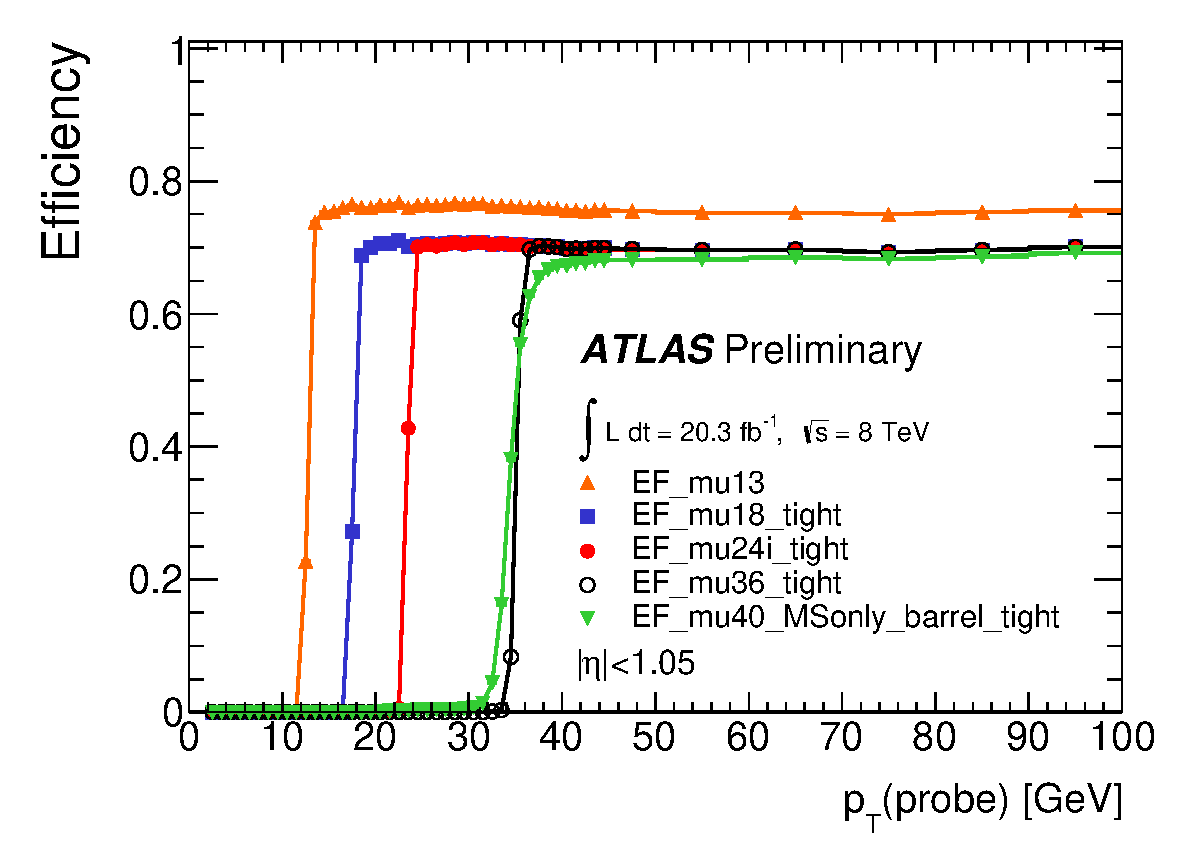
\includegraphics[width=0.495\textwidth]{tex/selection/trigger_eff_mu}
	\caption{Efficiencies of the single lepton triggers for electrons with respect to 
	offline \textit{medium} identification (left) and muons with respect to offline 
	reconstruction (right).}
	\label{fig:sel:trig_eff}
\end{figure}

Events are required to pass at least one trigger listed in \Table~\ref{tab:sel:triggers}. 
The single lepton triggers include a tighter low-\pt trigger and a looser high-\pt 
trigger in order to maximise the efficiency. Dilepton triggers are then used to increase 
the efficiency during the turn-on \pt of the single lepton triggers. These triggers 
collectively support a \pt threshold of \unit{22}{\GeV} on the leading lepton (in the 
offline analysis), whilst operating on the plateau.

\begin{table}
	\begin{tabular}{lllcl}
		\multirow{2}{2.5cm}{Single lepton triggers} & \Pe  & \verb|EF_e24vhi_medium1| & or & \verb|EF_e60_medium1| \\
		& \Pmu & \verb|EF_mu24i_tight| & or & \verb|EF_mu36_tight|  \\
		\hline
		\multirow{3}{2.5cm}{Dilepton triggers} & \HepProcess{\Pe\Pe} & \verb|EF_2e12Tvh_loose1| & or & \verb|EF_2e12Tvh_loose1_L2StarB| \\
		& \HepProcess{\Pmu\Pmu} & \multicolumn{3}{l}{\texttt{EF\symbol{95}mu18\symbol{95}tight\symbol{95}mu8\symbol{95}EFFS}} \\
		& \HepProcess{\Pe\Pmu}  & \multicolumn{3}{l}{\texttt{EF\symbol{95}e12Tvh\symbol{95}medium1\symbol{95}mu8}} \\
	\end{tabular}
	\caption{Employed trigger names. \texttt{EF} refers to event filter, \texttt{e} is an 
	electron, \texttt{mu} is a muon, the following number is the \pt threshold, 
	\texttt{vh} indicates calorimeter isolation, \texttt{i} indicates track isolation, 
	and \texttt{tight}, \texttt{medium} or \texttt{loose} is the identification. Other 
	parts relate to the trigger chain. Criteria are looser than those applied 
	offline.}
	\label{tab:sel:triggers}
\end{table}

Trigger efficiencies are measured via tag-and-probe of 
\HepProcess{\PZ \HepTo \Plepton\Plepton} events, where the tag and probe have both 
passed the offline lepton selection and the tag has successfully matched to a triggered 
lepton object. For example, single lepton trigger efficiencies are displayed in 
\Figure~\ref{fig:sel:trig_eff}. Comparison with MC yields efficiency scale factors.

Additionally, events are required to have at least one lepton passing the offline 
reconstruction that is matched within $\Delta R < 0.15$ of a triggered lepton object.
Single lepton triggers are matched to offline leptons with $\pt > \unit{25}{\GeV}$. On 
the other hand, dilepton triggers comprise two triggered objects: \texttt{mu8} is matched 
to offline muons with $\pt > \unit{10}{\GeV}$, \texttt{mu18} is matched to offline muons 
with $\pt > \unit{20}{\GeV}$, and \texttt{e12} is matched to offline electrons with 
$\pt > \unit{15}{\GeV}$.



\subsection{Inclusive preselection}
\label{sec:selection:presel}

\subsection{0-jet selection}
\label{sec:selection:0j}

\subsection{1-jet bin}
\label{sec:selection:1j}

\subsection{$\geq 2$-jet bin}
\label{sec:selection:2j}

\begin{table}
	\begin{tabular}{cc}
		\em/\me & \ee/\mm \\
		\hline
		\multicolumn{2}{c}{\ptleadlep $>$ \unit{22}{\GeV}} \\
		\mll $>$ \unit{10}{\GeV} & \mll $>$ \unit{12}{\GeV} \\
		-- & $\mods{\mll - \mZ} > $ \unit{15}{\GeV} \\
		\hline
		% 0 JET
		\multicolumn{2}{c}{0-jet selection} \\
		\hline
		\corrtrackmet $>$ \unit{20}{\GeV} & \metrel $>$ \unit{40}{\GeV} \\
		\multicolumn{2}{c}{\njets $=$ 0} \\
		\multicolumn{2}{c}{\dphillmet $> \pi/2$} \\
		\multicolumn{2}{c}{\ptll $>$ \unit{30}{\GeV}} \\
		\multicolumn{2}{c}{\mll $<$ \unit{55}{\GeV}} \\
		-- & \trackmet $>$ \unit{40}{\GeV} \\
		\multicolumn{2}{c}{\dphill $<$ 1.8} \\
		-- & \frecoil $<$ 0.1 \\
		\hline
		% 1 JET
		\multicolumn{2}{c}{1-jet selection} \\
		\hline
		\corrtrackmet $>$ \unit{10}{\GeV} & \metrel $>$ \unit{40}{\GeV} \\
		\multicolumn{2}{c}{\njets $=$ 1} \\
		\multicolumn{2}{c}{\nbjets $=$ 0} \\
		$\max\parenths{\mt{\Plepton_1}, \mt{\Plepton_2}} >$ \unit{50}{\GeV} & -- \\
		$m_{\Ptau\Ptau} < \mZ - \unit{25}{\GeV}$ & -- \\
		\multicolumn{2}{c}{\mll $<$ \unit{55}{\GeV}} \\
		-- & \trackmet $>$ \unit{35}{\GeV} \\
		\multicolumn{2}{c}{\dphill $<$ 1.8} \\
		-- & \frecoil $<$ 0.1 \\
	\end{tabular}
	\caption{Summary}
	\label{tab:selection}
\end{table}